\chapter{Teil von Prof. Dr. Ass. Roland Christen aka Surfer Boy}

\section{Persistenz}
Persistenz stammt aus dem lateinischen \emph{persistere} und steht für das langfristige Fortbestehen einer Sache. In der Informatik wollen wir das Fortbestehen der Daten sichern.

\subsection{Modellierung}
Die Datenmodellierung erfolgt auf drei Ebenen. Konzeption, Implementation und physischer Entwurf. In DMG haben wir den konzeptionellen Entwurf mittels ERM gemacht. In APPE lernen wir, dass dieser nicht Praxis tauglich ist und verwenden nun UML-Klassendiagramme (siehe Abbildung \ref{fig:konzeptionelles-datenmodell-mit-klassendiagram}).
\begin{figure}[h!]
\centering
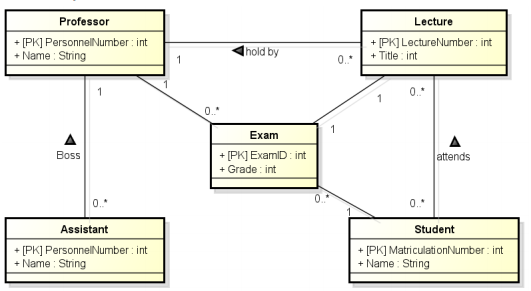
\includegraphics[width=0.7\linewidth]{fig/konzeptionelles-datenmodell-mit-klassendiagram}
\caption{Konzeptionelles Datenmodell mit UML Klassendiagrammen}
\label{fig:konzeptionelles-datenmodell-mit-klassendiagram}
\end{figure}
Nach der Konzeption folgt die Implementation. Der konzeptionelle Entwurf ist vollständig unabhängig von der konkreten Datenbank. Nun kann das konzeptionelle Modell für eine konkrete Datenbank transformiert werden. Bisher wählten wir immer relationale Datenbanken.
Ein Beispiel dafür sehen wir in Abbildung \ref{fig:relationales-datenmodell}.

\begin{figure}[h!]
\centering
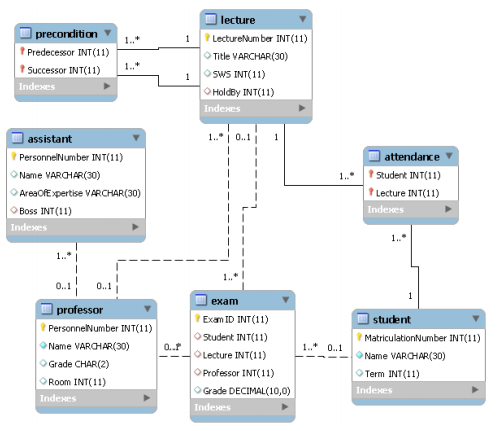
\includegraphics[width=0.7\linewidth]{fig/relationales-datenmodell}
\caption{Relationales Datenmodell}
\label{fig:relationales-datenmodell}
\end{figure}

\newpage

\subsection{JPA (Java Persistence API)}
Nun haben wir das effektive Schema, welches wir auf unserem DBMS installieren können. Nun wollen wir auf die Daten aus einem Java-Programm zugreifen.

Und hier müssen wir ein ORM durchführen. ORM steht für objekt-relationales Mapping. Darauf ist die Informatik nicht stolz und es gilt als notwendiges Übel. Eine ORM Architektur ist in der Abbildung \ref{fig:orm-basics} ersichtlich.

\begin{figure}[h!]
\centering
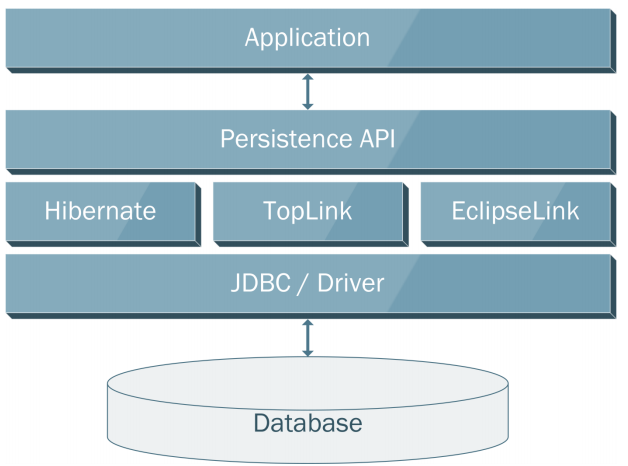
\includegraphics[width=0.5\linewidth]{fig/orm-basics}
\caption{ORM Basics}
\label{fig:orm-basics}
\end{figure}

\noindent
Folgendes sind Schlüsselelemente in JPA:
\begin{description}
	\item[Entity:] Java-Klasse, welche für eine Tabelle steht.
	\item[Annotation:] Definitionen für das OR Mapping (Beginnen mit @). Man kann auch das gesamte Mapping in XML Files definieren, aber eher Old-School und nicht fresh Surfer-like.
	\item[EntityManager:] Klasse um auf die Entities zuzugreifen.
	\item[Persistence Unit:] Konfiguration für DB-Verbindung, DB Treiber usw.
	\item[JPQL:] Java Persistence Query Language. Objektorienterte Abfragesprache. Abstrahiert SQL voll umfänglich!
\end{description}

\subsubsection{Vorgehen}
Entweder definiert man die Datenbanktabellen zuerst und generiert daraus die Entities oder man implementiert die Entities und generiert daraus die Datenbanktabellen. Christens Approach ist, dass man das Schema selber schreibt und die Entities daraus generiert. Wir gehen auch so vor. Es ist extrem wichtig, dass das Datenmodell korrekt ist und wir wollen hier uns nicht auf irgendwelche Tools verlassen. Ich will genau definieren wie die Zusammenhänge sind. Ausserdem will ich Herr sein über die Attribute in welcher Domäne mit welcher Konfiguration sie stecken. Anschliessend kann man die Entities generieren - man muss sich das Mapping danach nochmals anschauen!
Um die bestimmten Objekte zu generieren, gibt es verschiedene Tools. Die moderne IDEs besitzen solche Tools.

\subsubsection{Coding}
Abbildung \ref{fig:sample-jpa-code} zeigt ein Beispiel wie man das JPA verwendet. Die \texttt{EntityManagerFactory} ist teuer und sollte pro Run nur einmal instantiiert werden. Der \texttt{EntityManager} (not threadsafe), welcher man daraus holen kann ist leichtgewichtig und kann quasi pro Request erzeugt und wieder verworfen werden. P.S: Das ist genau das was in JavaEE passiert. Der EntityManager wird injected und zwar pro Request. Die EntityManagerFactory wird bei Applikationsstart erzeugt. Im Beispiel sehen wir auch, dass die Transaktionen manuell gestartet und geschlossen werden. In JavaEE wird das in der Regel vom Container übernommen. 

\begin{figure}[h!]
\centering
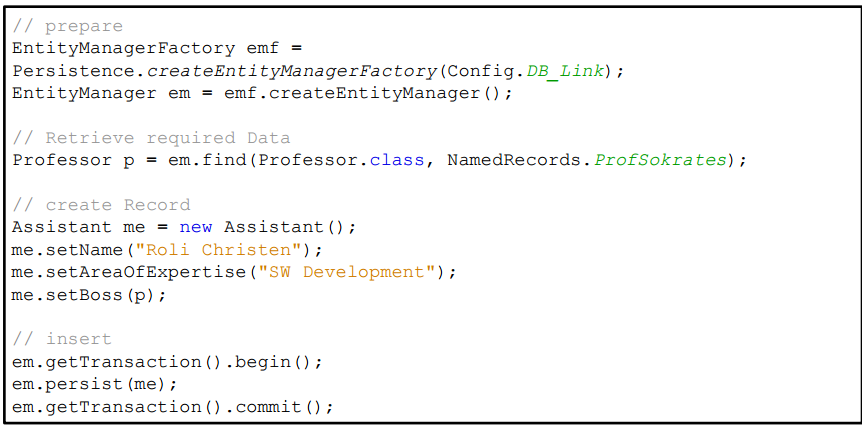
\includegraphics[width=0.8\linewidth]{fig/sample-jpa-code}
\caption{Beispiel Code JPA}
\label{fig:sample-jpa-code}
\end{figure}

Nachfolgend einige JPA-Methoden und Pitfalls:
\begin{itemize}
	\item em.remove(Entity e): Löschen einer Entity.
	\item persist vs merge: Persist inserted oder updated ein Entity und macht diese managed. Merge inserted oder updated eine Entity und macht diese aber nicht managed!
	\item managed (attached) vs unmanaged (dettached): Falls man mit einem managed Entity arbeitet und ein Attribut Wert ändert, wird dies direkt auf der Datenbank aktualisiert. Bei den unmanaged ist dies nicht der Fall und man muss nachträglich noch persist bzw. merge aufrufen.
\end{itemize}

\subsection{JPQL}
Dient um die Objekte mit einer objektorientierten Sprache abzufragen (siehe Abbildung \ref{fig:sample-jpql-code}. Wenn man JPQL verwendet, besteht immer die Gefahr, dass der String (JPQL Code) falsch geschrieben wurde. Passiert natürlich mit sauberem Testing nicht :). Trotzdem kann uns der Compiler hier nicht helfen und haben Code, welcher erst zur Runtime sein wahres Gesicht zeigt. Eine Alternative ist der CriteriaBuilder, welcher voll-typisierte Abfragen ermöglicht. Dieser ermöglicht es, dass wir keine ungültigen Abfragen schreiben!! Aber dieser scheint nicht Teil dieses Moduls zu sein.

\begin{figure}[h!]
\centering
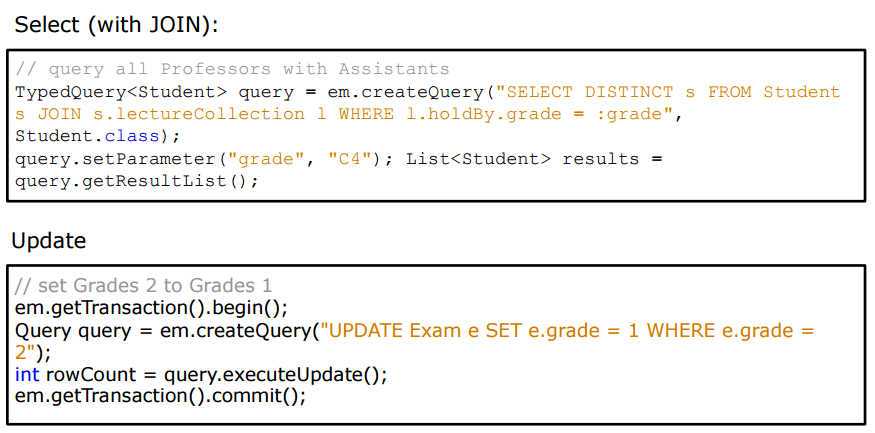
\includegraphics[width=0.8\linewidth]{fig/sample-jpql-code}
\caption{JPQL Code}
\label{fig:sample-jpql-code}
\end{figure}

\subsection{Caching}
Achtung der EntiyManager cached! Wenn ich die Liste aller Studenten eines Professors lade, anschliessend einen Student lösche und nochmals dieselbe Liste lade, können wieder dieselben Entities daherkommen. Man kann die Liste mittels em.refresh(List<?> list) aktualisieren. Oder Den Cache des EM mittels evictAll() löschen. Oder das Entity manuell aus der Liste löschen oder Framework Features verwenden wie \emph{orphanRemoval=true}.





